\documentclass[a4paper]{article}

\usepackage[margin=5mm]{geometry}
\usepackage{tikz,pgfplots}
\usetikzlibrary{matrix,backgrounds}
%\usetikzlibrary{matrix,arrows,calc,shadows,positioning,patterns,backgrounds}

\usepackage{mathtools}

\usepgfplotslibrary{external} % creates a tight self-contained pdf figure for each tikzpicture
\tikzexternalize % comment out to debug if latex errors: generates the external pdf
\tikzset{external/force remake} % force remarking of external pdf otherwise will use external pdf
\tikzsetexternalprefix{fig/} % output the pdf to an existing directory (needs to exist)

% sips: scriptable image processing system.
\tikzset{png export/.style={
	external/system call={
		pdflatex \tikzexternalcheckshellescape
			-halt-on-error -interaction=batchmode -jobname "\image" "\texsource";
		sips -s format png --out "\image.png" "\image.pdf";
		sips -s dpiWidth 600 -s dpiHeight 600 -s format png --out "\image-600.png" "\image.pdf";
		}}}

%6A9FB5 - Lanyon blue
%B5CFDA - Lanyon blue 50 : 50 White

\definecolor{rak-blue}{HTML}{DFEFDF}
\newcommand{\drawbackgroundframe}{
	\begin{pgfonlayer}{background}
		\draw[rak-blue!50!black,fill=rak-blue] (current bounding box.south west) rectangle
			(current bounding box.north east);
	\end{pgfonlayer}}

\pgfplotsset{compat=1.12}

\newcommand{\minibox}[1]{%
	\begin{minipage}[c]{30mm}\centering\large\sffamily #1\end{minipage}}

\newcommand{\dude}[2]{\minibox{\hbox to 30mm{\hss#1\hss} \bfseries #2}}

\tikzset{png export}

\begin{document}
\thispagestyle{empty}

\tikzsetnextfilename{rak-genealogy}

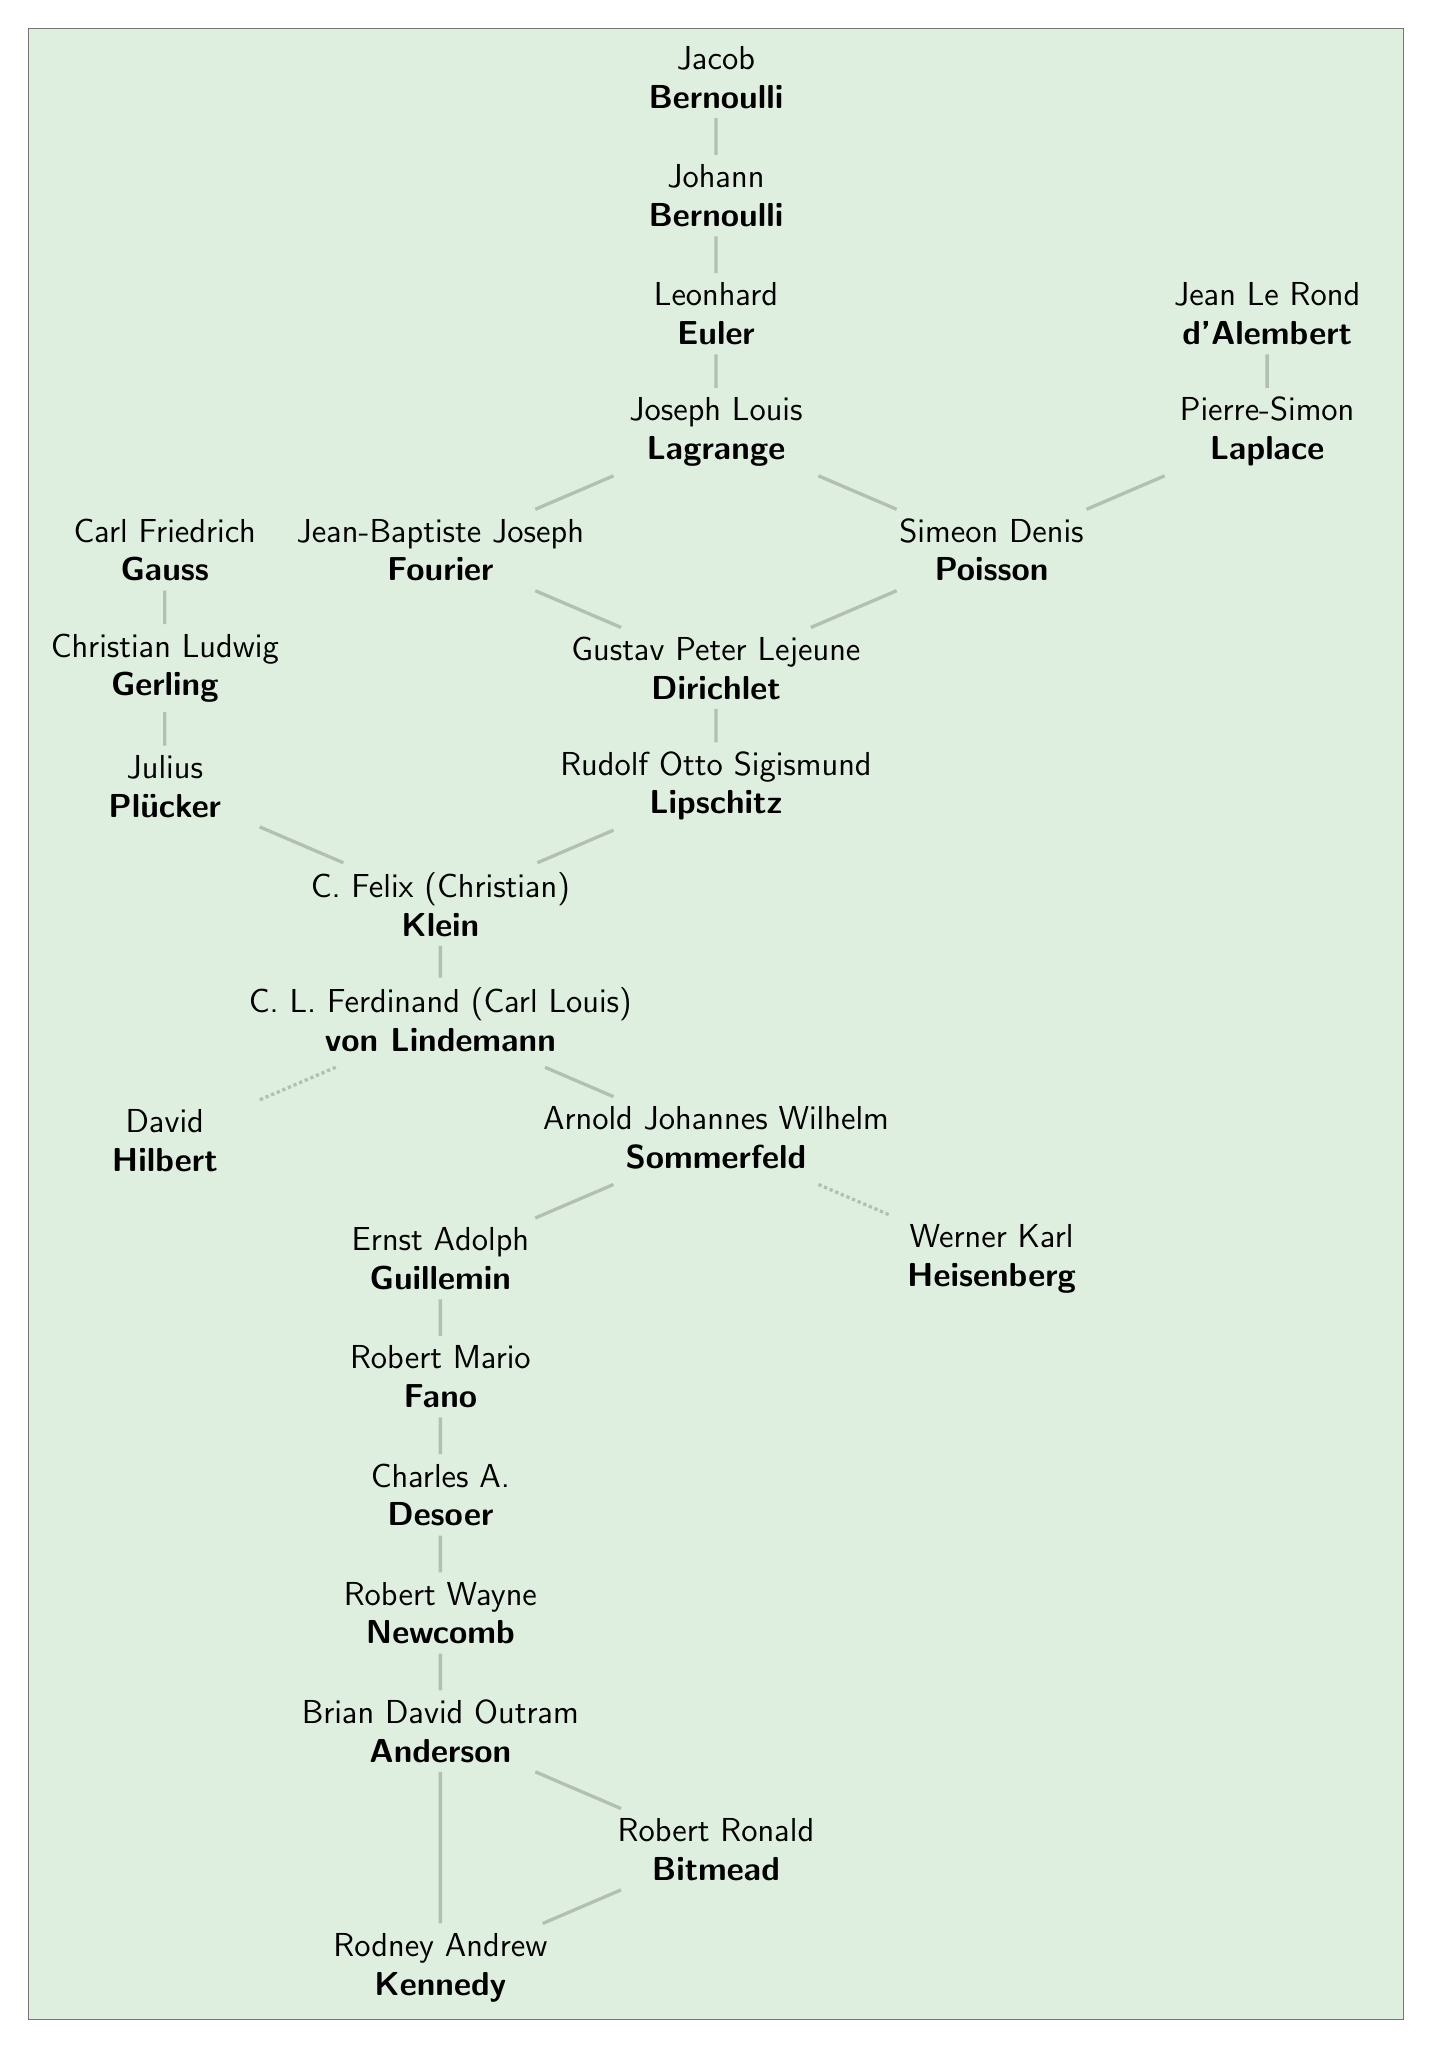
\begin{tikzpicture}
	\matrix (m) [matrix of math nodes,%ampersand replacement=\&,
		column sep={35mm,between origins}, row sep={15mm,between origins}]{
		& & \dude{Jacob}{Bernoulli} & & \\
		& & \dude{Johann}{Bernoulli} \\
		& & \dude{Leonhard}{Euler} & & \dude{Jean Le Rond}{d'Alembert} \\
		& & \dude{Joseph Louis}{Lagrange} & & \dude{Pierre-Simon}{Laplace} \\
		\dude{Carl Friedrich}{Gauss} & \dude{Jean-Baptiste Joseph}{Fourier} & & \dude{Simeon Denis}{Poisson} \\
		\dude{Christian Ludwig}{Gerling} & & \dude{Gustav Peter Lejeune}{Dirichlet} \\
		\dude{Julius}{Pl\"ucker} & & \dude{Rudolf Otto Sigismund}{Lipschitz} \\
		& \dude{C. Felix (Christian)}{Klein} \\
		& \dude{C. L. Ferdinand (Carl Louis)}{von Lindemann\vphantom{g}} \\
		\dude{David}{Hilbert} & & \dude{Arnold Johannes Wilhelm}{Sommerfeld\vphantom{g}} \\
		& \dude{Ernst Adolph}{Guillemin} && \dude{Werner Karl}{Heisenberg}\\
		& \dude{Robert Mario}{Fano} \\
		& \dude{Charles A.}{Desoer} \\
		& \dude{Robert Wayne}{Newcomb} \\
		& \dude{Brian David Outram}{Anderson} \\
		& & \dude{Robert Ronald}{Bitmead} \\
		& \dude{Rodney Andrew}{Kennedy} \\
	};
	\begin{scope}[very thick, rak-blue!80!black]
		\draw (m-5-1) -- (m-6-1) -- (m-7-1) -- (m-8-2) -- (m-9-2) ;
		\draw [densely dotted] (m-9-2) -- (m-10-1) (m-10-3) -- (m-11-4);
		\draw (m-1-3) -- (m-2-3) -- (m-3-3) -- (m-4-3) -- (m-5-4);
		\draw (m-4-3) -- (m-5-2) -- (m-6-3) -- (m-7-3) -- (m-8-2);
		\draw (m-3-5) -- (m-4-5) -- (m-5-4) -- (m-6-3);
		\draw (m-9-2) -- (m-10-3) -- (m-11-2) -- (m-12-2) -- (m-13-2) -- (m-14-2) -- (m-15-2) -- (m-17-2);
		\draw (m-15-2) -- (m-16-3) -- (m-17-2);
	\end{scope}
	\drawbackgroundframe
\end{tikzpicture}

\end{document}
